\section{Video analysis}

video=2D Dims+time Dim

\subsection{Problems: Videos are Big}

数据量太过庞大

SD (640 x 480): ~1.5 GB per minute
HD (1920 x 1080): ~10 GB per minute

Solution: Train on short clips, low fps and low spatial resolution
e.g. T = 16, H=W=112 (3.2 seconds at 5 fps, 588 KB)

\subsection{Video Classification: Single-Frame CNN}

Simple idea: 训练 2D CNN 分类视频每一帧, 然后取平均.

这在 video classification 的类别差异比较大的时候, 是一个很强的 baseline

\subsection{Video Classification: Late Fusion with FC}

\begin{figure}[htbp]
    \centering
    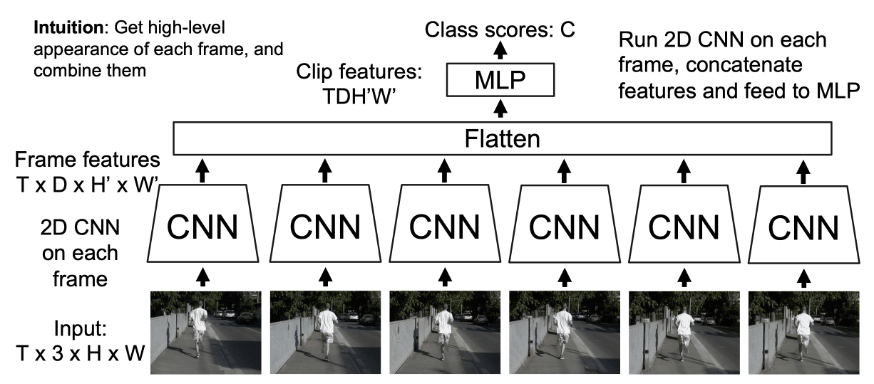
\includegraphics[scale=0.25]{figures/LF_FC.png}
    \caption{Late Fusion with FC}
\end{figure}

看得出来正着走和倒着走的区别吗? 可以看出来. Concatenate 是有顺序的, 但是没有使用时间 equalvariance 的信息.

\subsection{Video Classification: Late Fusion with Pooling}

\begin{figure}[htbp]
    \centering
    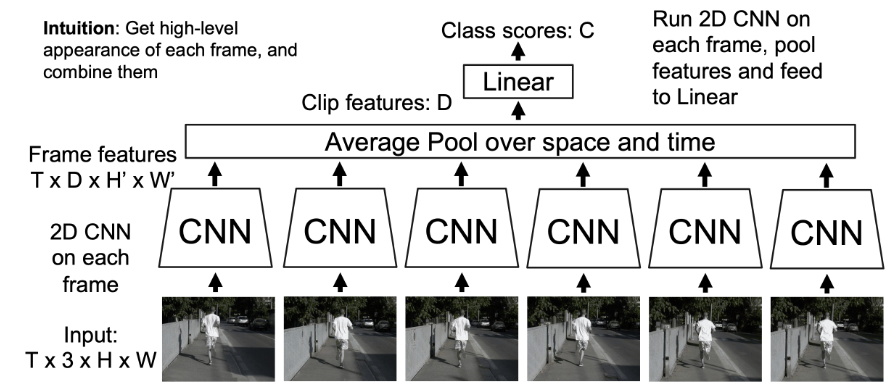
\includegraphics[scale=0.25]{figures/LF_pool.png}
    \caption{Late Fusion with Pooling}
\end{figure}

看得出来正着走和倒着走的区别吗? 看不出来

看得出来跑和走的区别吗? 看得出来,分辨重心feature.

更好得区分跑和走? 使用MaxPool, 在fusion的时候不要模糊所有帧的特征

\subsection{Video Classification: Early Fusion}

\begin{figure}[htbp]
    \centering
    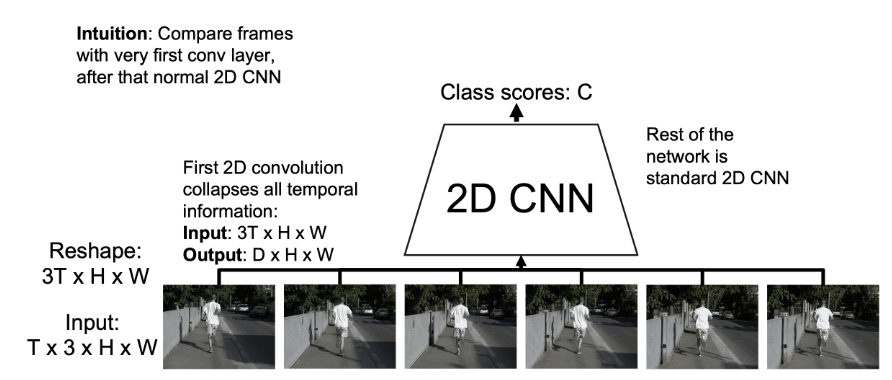
\includegraphics[scale=0.25]{figures/EF.png}
    \caption{Early Fusion}
\end{figure}

early fusion:所有时间信息在第一步提取,难度较高

所以一层处理时间信息可能不够

\subsection{Video Classification: 3D CNN}

\begin{figure}[htbp]
    \centering
    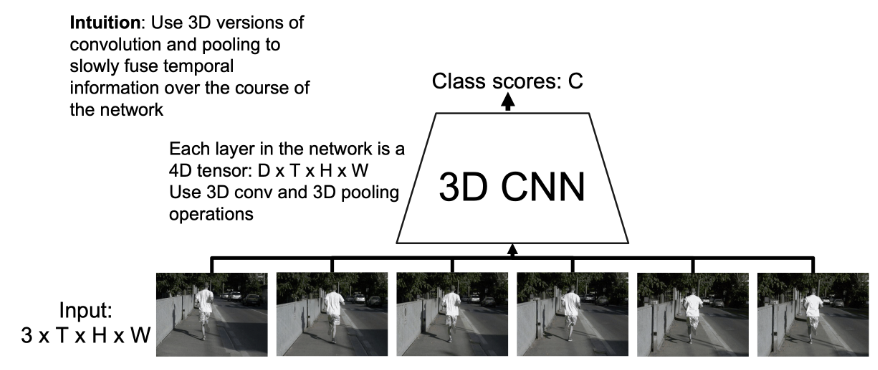
\includegraphics[scale=0.25]{figures/3DCNN.png}
    \caption{3D CNN}
\end{figure}

3D CNN将时间视作第三个空间维度.但问题在于:这对感受野的要求比较大.

在视频当中,
一件事情的效应可能在相当长的时间之后才能体现,而3D CNN在各个维度感受野的增长又比较均匀,
$3\times3$的时间维度卷积可能远远不如$3\times3$的图片卷积对于最终的分类结果用处大,
从这里可以看出,在视频处理当中,空间范围和时间范围地位并不对等.
但CNN也不可能cover任意长的时间序列,这就是3DCNN的局限性.

到目前为止,我们的所有时3DCNN仅在大约2-5秒的视频片段中建模帧之间的局部运动,无法提取长期结构特征.

\subsection{Comparison}

\begin{figure}[htbp]
    \centering
    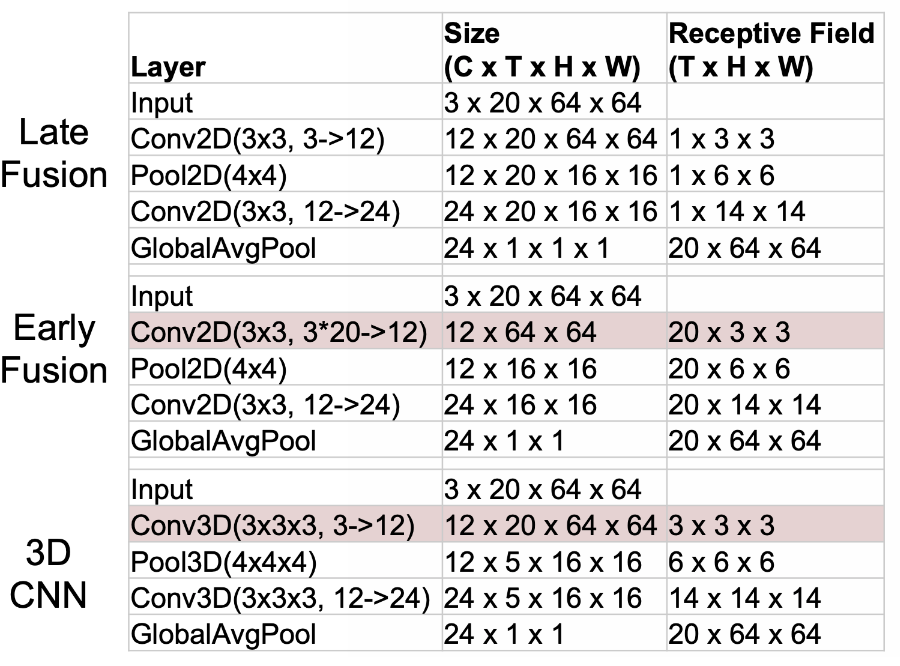
\includegraphics[scale=0.35]{figures/video_cmp.png}
    \caption{Video analysis method comparison}
\end{figure}

3D CNN 与 2D CNN 相比, 把卷积核扩展到时间维度, 感受野在时间维度上也是逐渐增大的.

更重要的是Late Fusion或者Early Fusion是没有办法处理时间局部信息的, 
3D CNN是可以处理时间局部信息的, 因为它有时间维度上的卷积操作.

\begin{itemize}
    \item Late Fusion: Build slowly in space, All-at-once in time at end
    \item Early Fusion: Build slowly in space, All-at-once in time at start
    \item 3D CNN: Build slowly in space, Build slowly in time "Slow Fusion"
\end{itemize}

\subsection{C3D: The VGG of 3D CNNs}

C3D: The VGG of 3D CNNs.第一次pool没有在时间维上处理,不希望提取得太早.

3d的kernel size比较敏感,$5^3 > 11^2$.移动多了一个维度,
计算代价更大.得益于其网络的精良设计,
C3D在 sports-1m 数据集上的top5 acc还是达到了84\%.

Problem: 3x3x3 conv is very expensive!

人类识别运动的关键:Motion,不是pixel.

Use Both Motion and appearance: two-stream fusion network.它使用经典算法获得flow输入神经网络.
神经网络分为两支,一支做空间,一支做时间.时间(flow)这一支使用了early fusion,因为相对于RGB,光流的信息已经比较清晰.

\subsection{Modeling Long-Term Temporal Structure}

我们希望处理序列,RNN如何? aggregation(聚合).

CNN和RNN一起训练计算代价太大.
因此先train CNN,不向其传递梯度,只训练RNN.但这样CNN与RNN可能优化目标不同.

如何 pre-train? 使用ImagenNet不好, 因为ImageNet的分类和Sports1M的分类粒度不同.

end to end training:端到端训练.所有optimization variable同时被优化.

\subsection{Recurrent convolutional Network}

\begin{figure}[htbp]
    \centering
    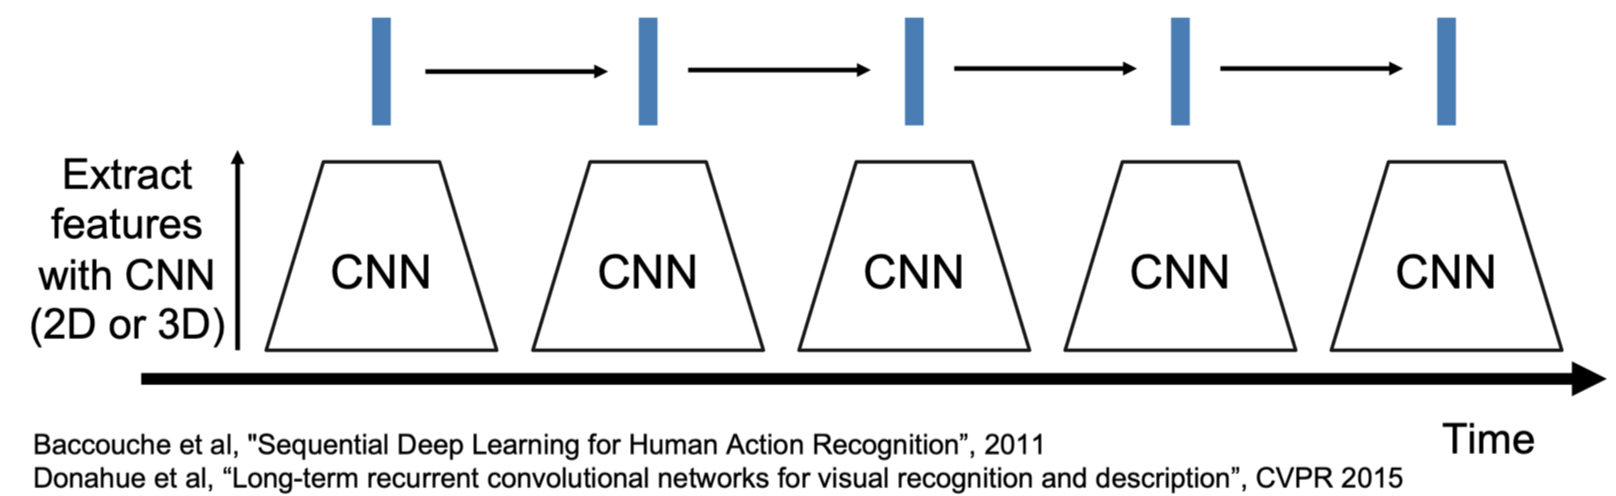
\includegraphics[scale=0.2]{figures/recur_CNN.png}
    \caption{Recurrent Convolutional Network}
\end{figure}

\begin{itemize}
    \item 在CNN中每个值是固定时间帧(代表了局部时间结构)的函数 
    \item 在RNN中每个向量是所有先前向量(代表了全局时间结构)的函数
\end{itemize}

把这两个网络合并起来?

\begin{figure}[H]
    \centering
    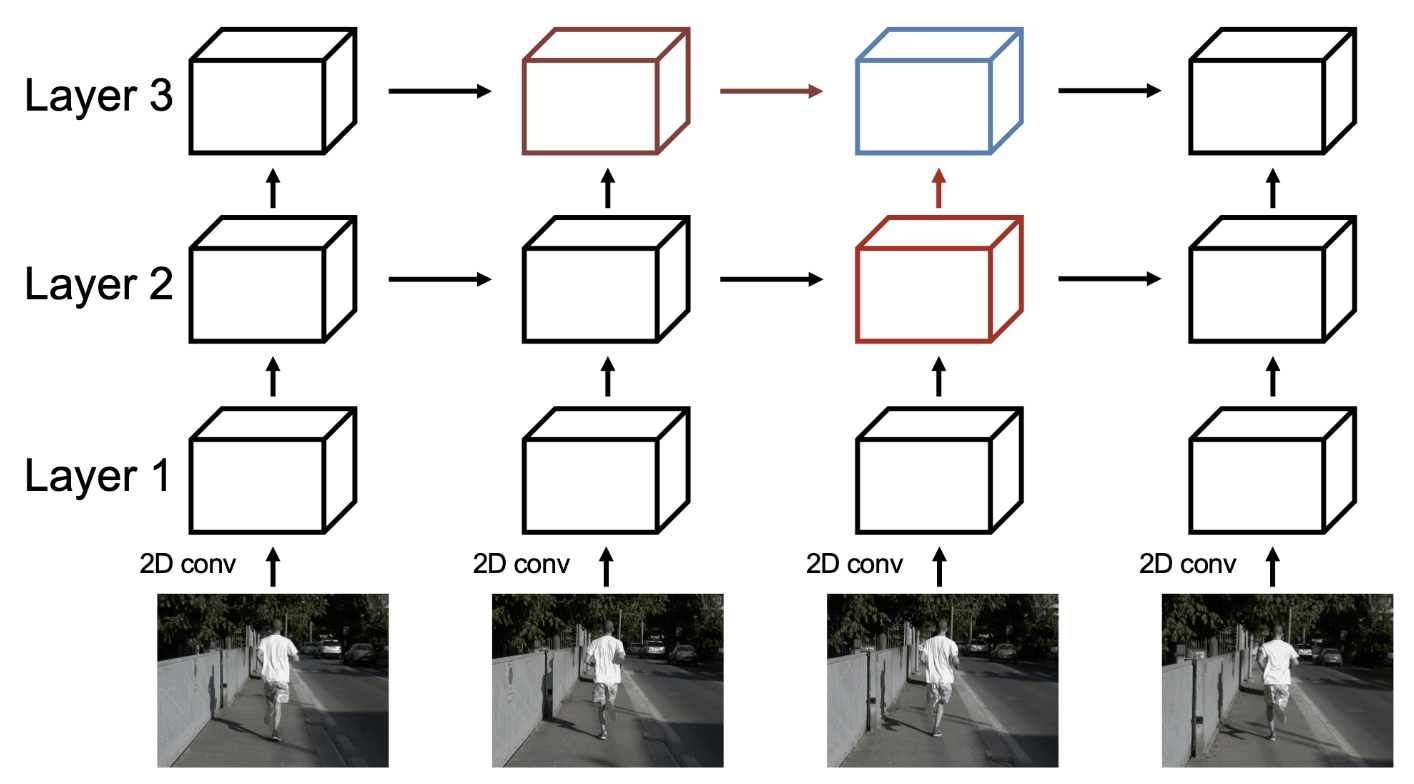
\includegraphics[scale=0.2]{figures/recu_CNN.png}
    \caption{Recurrent convolutional Network}
\end{figure}

每层依赖于两个输入
\begin{itemize}
    \item 同层,前一个时间步
    \item 前一层,同一个时间步
\end{itemize}

\begin{figure}[H]
    \centering
    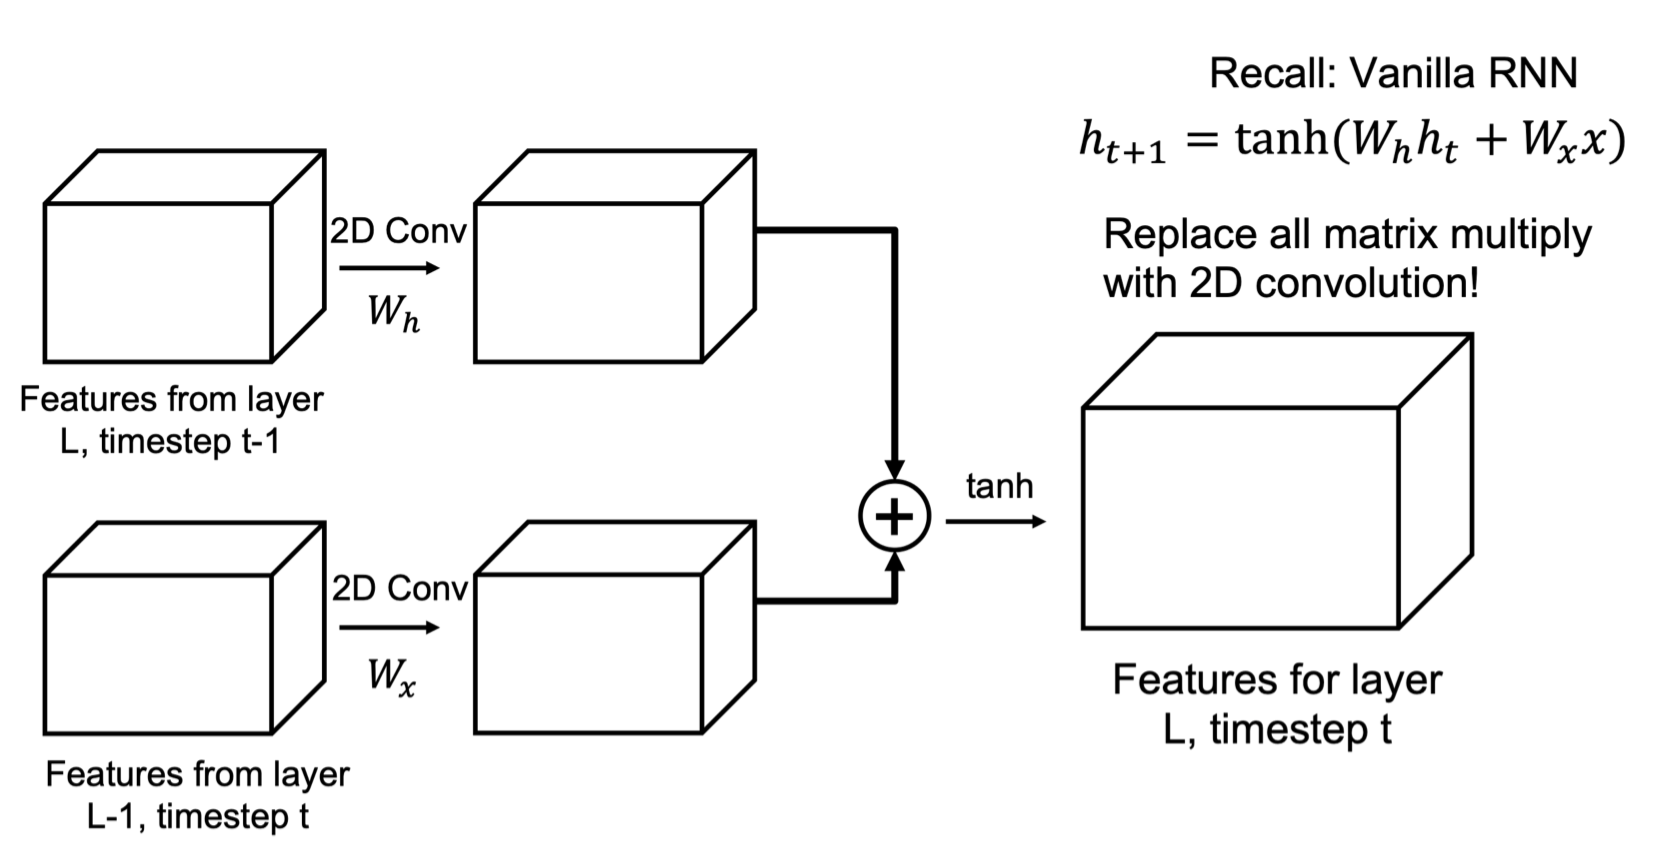
\includegraphics[scale=0.2]{figures/recur_CNN_detail.png}
    \caption{How to combine CNN and RNN}
\end{figure}

在每一层使用不同的权重,在时间上共享权重

问题在于循环神经网络不能并行训练,因此训练很慢.

跟 3D CNN 区别: 3D CNN 不是 recurrent 的, 是被3D卷积核决定的一个固定长度, 
而 recurrent convolutional network 是一个 recurrent network, 可以读取到之前所有的信息.
